%!TEX root = ../thesis.tex

\section{再帰型ニューラルネットワーク}
再帰型ニューラルネットワーク(Recurrent Neural Network, RNN)\cite{rumelhart1986learning1,rumelhart1986learning2}は,時系列データや系列データを扱うために設計されたニューラルネットワークの一種である.隠れ層の出力を次の時間ステップの入力として再利用し,データの時間的依存性をモデル化できる点が特徴である.この仕組みにより,従来は困難だった順序情報の学習が可能となる.

RNNは,入力層・隠れ層・出力層から構成される.
時系列データでは,各時刻の入力が順次RNNに与えられ,\figref{Fig:rnn}のように隠れ層が現在の入力と直前の隠れ状態を組み合わせて次の隠れ状態を生成する.この隠れ層が過去の情報を保持し,長期依存関係の学習を担う.数式で表すと,時刻$t$における隠れ状態$h_t$は式\eqref{rnn}のように計算される.
\begin{equation}
h_t = f(W_{xh}x_t + W_{hh}h_{t-1} + b_n)\label{rnn}
\end{equation}
ここで,$x_t$は時刻$t$の入力,$h_{t-1}$は時刻$t-1$の隠れ状態,$W_{xh}$と$W_{hh}$はそれぞれ入力重みと隠れ層の重み行列,$b_n$はバイアス項,そして$f$は非線形活性化関数である.

RNNには,時間の経過とともに勾配が減少または増大し続けることで学習が困難になる勾配消失問題\cite{hochreiter2001gradient-grad,weinleindiplomarbeit-grad,schmidhuber2015deep-grad}や勾配爆発問題が存在する.これらの問題は,長い系列データを扱う場合に十分な長期依存性を学習できない原因となる.そこで,LSTM(Long Short Term Memory)\cite{hochreiter1997long}やGRU(Gated Recurrent Unit)\cite{chung2014empirical-gru}などの改良モデルが提案されている.これらのモデルは,ゲート機構を用いて重要な情報を選択的に保持または忘却することで,長期依存性を効率よく学習するように設計されている.
% \vspace{-10pt}
\begin{figure}[hbtp]
  \centering
 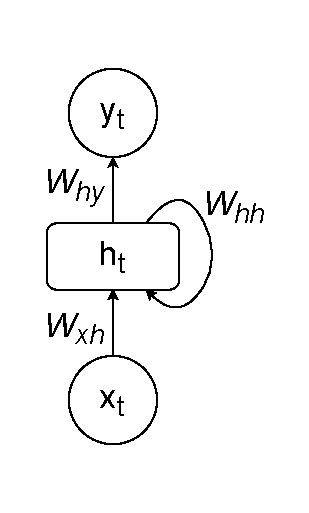
\includegraphics[keepaspectratio, scale=0.52]
      {images/neural-network-rnn.pdf}
 \caption{Recurrent neural network}
 \label{Fig:rnn}
\end{figure}   

\newpage
